\title{Ensemble methods for Yelp review classification}
\author{Shayan Ali Akbar\\ \small sakbar@purdue.edu\\ \small CS 57300 Homework 4\\
	This is one day late submission.}
\date{}

\documentclass[12pt]{article}
\usepackage{amsmath}
\usepackage[boxruled,linesnumbered]{algorithm2e}
\usepackage{xcolor}
\usepackage{graphicx}

\newcommand\mycommfont[1]{\footnotesize\ttfamily\textcolor{black}{#1}}
\SetCommentSty{mycommfont}

\addtolength{\oddsidemargin}{-.875in}
\addtolength{\evensidemargin}{-.875in}
\addtolength{\textwidth}{1.75in}
\addtolength{\topmargin}{-1.0in}
\addtolength{\textheight}{2.2in}
\pagenumbering{gobble}

\begin{document}
\maketitle

\newpage

\section{Introduction}

In this report we discuss the five very popular classifiers for the task of yelp review
classification. In particular we discuss the support vector machines, decision trees,
bagged decision trees, random forests, and boosted decision trees.

The report is organised as follows. The next four sections deal with the Analysis 1,
Analysis 2, Analysis 3, and Analysis 4 of the homework 4 handout. Finally in the last
section we discuss the Boosted decision trees.

\section{Analysis 1}

\subsection{Learning Curves}
The plot of results is shown in Figure 1. On x-axis we vary the training set sizes. Instead
of percents, we have plotted the actual number of training set examples used to learn
the model. On y-axis is the zero one loss. We have three plots --- one for each model.
The different colored plots belong to different models as indicated in the legend.
The vertical bars show the standard error calculated as
described in the homework handout. The values of zero one loss for each of the six 
training set size averaged accross 10 fold are shown in the figure.

These average and standard error values are calculated from the following zero
one loss values calculated for each model for training set size for each of the 10 folds.
Notice that the horizontal = bar separated the results for each training set size. The
zero one losses present within two horizontal = bars belong to the different folds for
a specific training set size.\\

\noindent=======================================\\
ZERO-ONE-LOSS-DT 0.385
ZERO-ONE-LOSS-BT 0.48
ZERO-ONE-LOSS-RF 0.54
ZERO-ONE-LOSS-BS 0.44
ZERO-ONE-LOSS-SVM 0.24
ZERO-ONE-LOSS-DT 0.485
ZERO-ONE-LOSS-BT 0.34
ZERO-ONE-LOSS-RF 0.34
ZERO-ONE-LOSS-BS 0.3
ZERO-ONE-LOSS-SVM 0.25
ZERO-ONE-LOSS-DT 0.355
ZERO-ONE-LOSS-BT 0.4
ZERO-ONE-LOSS-RF 0.4
ZERO-ONE-LOSS-BS 0.3
ZERO-ONE-LOSS-SVM 0.22
ZERO-ONE-LOSS-DT 0.28
ZERO-ONE-LOSS-BT 0.24
ZERO-ONE-LOSS-RF 0.28
ZERO-ONE-LOSS-BS 0.26
ZERO-ONE-LOSS-SVM 0.235
ZERO-ONE-LOSS-DT 0.31
ZERO-ONE-LOSS-BT 0.18
ZERO-ONE-LOSS-RF 0.2
ZERO-ONE-LOSS-BS 0.2
ZERO-ONE-LOSS-SVM 0.13
ZERO-ONE-LOSS-DT 0.39
ZERO-ONE-LOSS-BT 0.32
ZERO-ONE-LOSS-RF 0.24
ZERO-ONE-LOSS-BS 0.34
ZERO-ONE-LOSS-SVM 0.18
ZERO-ONE-LOSS-DT 0.4
ZERO-ONE-LOSS-BT 0.38
ZERO-ONE-LOSS-RF 0.38
ZERO-ONE-LOSS-BS 0.26
ZERO-ONE-LOSS-SVM 0.17
ZERO-ONE-LOSS-DT 0.405
ZERO-ONE-LOSS-BT 0.32
ZERO-ONE-LOSS-RF 0.32
ZERO-ONE-LOSS-BS 0.2
ZERO-ONE-LOSS-SVM 0.19
ZERO-ONE-LOSS-DT 0.315
ZERO-ONE-LOSS-BT 0.24
ZERO-ONE-LOSS-RF 0.26
ZERO-ONE-LOSS-BS 0.2
ZERO-ONE-LOSS-SVM 0.225
ZERO-ONE-LOSS-DT 0.38
ZERO-ONE-LOSS-BT 0.44
ZERO-ONE-LOSS-RF 0.4
ZERO-ONE-LOSS-BS 0.24
ZERO-ONE-LOSS-SVM 0.255\\
=======================================\\
ZERO-ONE-LOSS-DT 0.325
ZERO-ONE-LOSS-BT 0.36
ZERO-ONE-LOSS-RF 0.36
ZERO-ONE-LOSS-BS 0.26
ZERO-ONE-LOSS-SVM 0.15
ZERO-ONE-LOSS-DT 0.35
ZERO-ONE-LOSS-BT 0.28
ZERO-ONE-LOSS-RF 0.32
ZERO-ONE-LOSS-BS 0.26
ZERO-ONE-LOSS-SVM 0.14
ZERO-ONE-LOSS-DT 0.335
ZERO-ONE-LOSS-BT 0.14
ZERO-ONE-LOSS-RF 0.28
ZERO-ONE-LOSS-BS 0.14
ZERO-ONE-LOSS-SVM 0.11
ZERO-ONE-LOSS-DT 0.295
ZERO-ONE-LOSS-BT 0.22
ZERO-ONE-LOSS-RF 0.24
ZERO-ONE-LOSS-BS 0.1
ZERO-ONE-LOSS-SVM 0.145
ZERO-ONE-LOSS-DT 0.325
ZERO-ONE-LOSS-BT 0.26
ZERO-ONE-LOSS-RF 0.26
ZERO-ONE-LOSS-BS 0.24
ZERO-ONE-LOSS-SVM 0.13
ZERO-ONE-LOSS-DT 0.29
ZERO-ONE-LOSS-BT 0.18
ZERO-ONE-LOSS-RF 0.2
ZERO-ONE-LOSS-BS 0.12
ZERO-ONE-LOSS-SVM 0.125
ZERO-ONE-LOSS-DT 0.23
ZERO-ONE-LOSS-BT 0.12
ZERO-ONE-LOSS-RF 0.26
ZERO-ONE-LOSS-BS 0.1
ZERO-ONE-LOSS-SVM 0.11
ZERO-ONE-LOSS-DT 0.425
ZERO-ONE-LOSS-BT 0.1
ZERO-ONE-LOSS-RF 0.22
ZERO-ONE-LOSS-BS 0.18
ZERO-ONE-LOSS-SVM 0.16
ZERO-ONE-LOSS-DT 0.35
ZERO-ONE-LOSS-BT 0.26
ZERO-ONE-LOSS-RF 0.26
ZERO-ONE-LOSS-BS 0.2
ZERO-ONE-LOSS-SVM 0.12
ZERO-ONE-LOSS-DT 0.29
ZERO-ONE-LOSS-BT 0.16
ZERO-ONE-LOSS-RF 0.26
ZERO-ONE-LOSS-BS 0.12
ZERO-ONE-LOSS-SVM 0.135\\
=======================================\\
ZERO-ONE-LOSS-DT 0.26
ZERO-ONE-LOSS-BT 0.24
ZERO-ONE-LOSS-RF 0.3
ZERO-ONE-LOSS-BS 0.16
ZERO-ONE-LOSS-SVM 0.08
ZERO-ONE-LOSS-DT 0.295
ZERO-ONE-LOSS-BT 0.22
ZERO-ONE-LOSS-RF 0.06
ZERO-ONE-LOSS-BS 0.1
ZERO-ONE-LOSS-SVM 0.07
ZERO-ONE-LOSS-DT 0.375
ZERO-ONE-LOSS-BT 0.18
ZERO-ONE-LOSS-RF 0.32
ZERO-ONE-LOSS-BS 0.16
ZERO-ONE-LOSS-SVM 0.105
ZERO-ONE-LOSS-DT 0.18
ZERO-ONE-LOSS-BT 0.22
ZERO-ONE-LOSS-RF 0.16
ZERO-ONE-LOSS-BS 0.2
ZERO-ONE-LOSS-SVM 0.125
ZERO-ONE-LOSS-DT 0.175
ZERO-ONE-LOSS-BT 0.12
ZERO-ONE-LOSS-RF 0.04
ZERO-ONE-LOSS-BS 0.08
ZERO-ONE-LOSS-SVM 0.095
ZERO-ONE-LOSS-DT 0.26
ZERO-ONE-LOSS-BT 0.26
ZERO-ONE-LOSS-RF 0.16
ZERO-ONE-LOSS-BS 0.16
ZERO-ONE-LOSS-SVM 0.09
ZERO-ONE-LOSS-DT 0.21
ZERO-ONE-LOSS-BT 0.16
ZERO-ONE-LOSS-RF 0.1
ZERO-ONE-LOSS-BS 0.1
ZERO-ONE-LOSS-SVM 0.095
ZERO-ONE-LOSS-DT 0.29
ZERO-ONE-LOSS-BT 0.16
ZERO-ONE-LOSS-RF 0.12
ZERO-ONE-LOSS-BS 0.12
ZERO-ONE-LOSS-SVM 0.105
ZERO-ONE-LOSS-DT 0.19
ZERO-ONE-LOSS-BT 0.16
ZERO-ONE-LOSS-RF 0.08
ZERO-ONE-LOSS-BS 0.1
ZERO-ONE-LOSS-SVM 0.11
ZERO-ONE-LOSS-DT 0.25
ZERO-ONE-LOSS-BT 0.22
ZERO-ONE-LOSS-RF 0.1
ZERO-ONE-LOSS-BS 0.16
ZERO-ONE-LOSS-SVM 0.085\\
=======================================\\
ZERO-ONE-LOSS-DT 0.28
ZERO-ONE-LOSS-BT 0.16
ZERO-ONE-LOSS-RF 0.24
ZERO-ONE-LOSS-BS 0.16
ZERO-ONE-LOSS-SVM 0.065
ZERO-ONE-LOSS-DT 0.205
ZERO-ONE-LOSS-BT 0.12
ZERO-ONE-LOSS-RF 0.3
ZERO-ONE-LOSS-BS 0.1
ZERO-ONE-LOSS-SVM 0.08
ZERO-ONE-LOSS-DT 0.13
ZERO-ONE-LOSS-BT 0.12
ZERO-ONE-LOSS-RF 0.04
ZERO-ONE-LOSS-BS 0.08
ZERO-ONE-LOSS-SVM 0.085
ZERO-ONE-LOSS-DT 0.19
ZERO-ONE-LOSS-BT 0.14
ZERO-ONE-LOSS-RF 0.16
ZERO-ONE-LOSS-BS 0.1
ZERO-ONE-LOSS-SVM 0.08
ZERO-ONE-LOSS-DT 0.215
ZERO-ONE-LOSS-BT 0.1
ZERO-ONE-LOSS-RF 0.12
ZERO-ONE-LOSS-BS 0.06
ZERO-ONE-LOSS-SVM 0.085
ZERO-ONE-LOSS-DT 0.22
ZERO-ONE-LOSS-BT 0.2
ZERO-ONE-LOSS-RF 0.08
ZERO-ONE-LOSS-BS 0.06
ZERO-ONE-LOSS-SVM 0.09
ZERO-ONE-LOSS-DT 0.165
ZERO-ONE-LOSS-BT 0.08
ZERO-ONE-LOSS-RF 0.12
ZERO-ONE-LOSS-BS 0.02
ZERO-ONE-LOSS-SVM 0.055
ZERO-ONE-LOSS-DT 0.26
ZERO-ONE-LOSS-BT 0.26
ZERO-ONE-LOSS-RF 0.22
ZERO-ONE-LOSS-BS 0.06
ZERO-ONE-LOSS-SVM 0.06
ZERO-ONE-LOSS-DT 0.18
ZERO-ONE-LOSS-BT 0.18
ZERO-ONE-LOSS-RF 0.14
ZERO-ONE-LOSS-BS 0.04
ZERO-ONE-LOSS-SVM 0.055
ZERO-ONE-LOSS-DT 0.285
ZERO-ONE-LOSS-BT 0.22
ZERO-ONE-LOSS-RF 0.32
ZERO-ONE-LOSS-BS 0.04
ZERO-ONE-LOSS-SVM 0.09


\begin{figure}
	\centering
	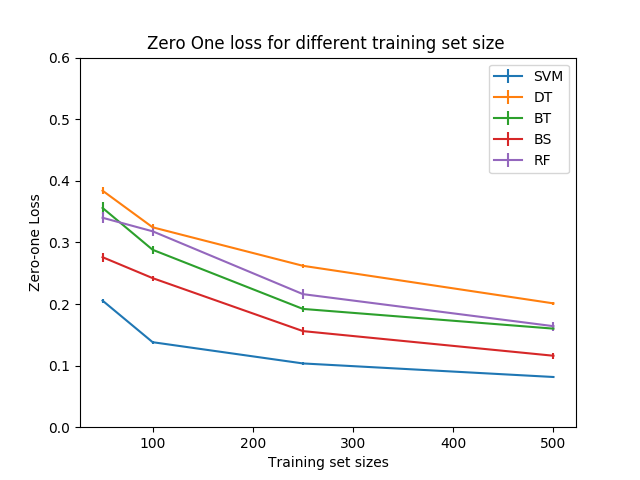
\includegraphics{Analysis1.png}
\end{figure}

\subsection{Hypothesis}

Let's compare the two algorithms SVM and Bagged Decision Trees (BT). 

Null hypothesis is that the SVM and BT are equivalent in terms of performance. It is assumed
to be true. So null hypothesis is the mean of SVM 0/1 losses is equivalent to mean of BT 0/1 losses. 
While the alternative hypothesis is that SVM and BT zero one losses are significantly different.
Or, the mean of SVM 0/1 losses is lesser than BT 0/1 losses.

\subsection{Discussion to test the hypothesis}

It is obvious from the plot of Figure 1 of average zero one losses and standard errors of the two
algorithms (SVM and BT) that their performances are very different from each other. This is because
in none of the training set sizes the error bars in the plot for the two algorithms are overlapping
each other as the plots are very far apart from each other.

To confirm this we perform paired t-test to compare their performances and to figure out whether
the differences between performances are statistically significant. The t-test are performed using
python statistics toolbox called scipy. Following are the results for each training set size.\\

For 2.5\% training set size:
  The two-tailed P value equals 0.0010. \\

For 5\% training set size:
  The two-tailed P value equals 0.0100. \\

For 12.5\% training set size:
  The two-tailed P value equals 0.0002.  \\

For 25\% training set size:
  The two-tailed P value equals 0.0021.\\

The average of alpha = 0.05 is 0.05 / 4 = 0.0125.

The null hypothesis is rejected since all p is less than 0.0125. In all the cases null is rejected.

It can also be seen from the graph that SVM being a non parametric model is significantly outperforming
the parametric models (DT and ensembles) when the size of training set is very low (100). 
While this difference is not that significant when the training set size is increased to 500.
May be if the training set size is further improved the ensembles will outperform SVM.

\section{Analysis 2}

\subsection{Learning Curves}

In this analysis we vary the feature set size --- the number of words to consider while building
the model. The comparative result while varying number of features is shown in Figure 2.

 On x-axis we vary the feature set sizes. On y-axis is the zero one loss. 
We have five plots --- one for each model with different color. The vertical 
bars show the standard error calculated as described in the homework handout. The 
values of zero one loss for each of the four feature set size averaged accross 10 fold for 
each of the five models along with the corresponding standard errors are given below. The
first array shows the average 0/1 losses while the second array shows the corresponding 
standard errors.
\\

=======SVM======

[0.1465, 0.095, 0.07699999999999999, 0.0705]

[0.0024191940806805893, 0.0019235384061671347, 0.0020396078054371138, 0.0022073740054644117]

=======DT======

[0.251, 0.2165, 0.23350000000000004, 0.2265]

[0.0028965496715920476, 0.0043763569324267882, 0.0039309668022001918, 0.0044724154547626724]

=======BT======

[0.20999999999999996, 0.176, 0.19, 0.20400000000000001]

[0.0045825756949558405, 0.0072553428588868225, 0.0050793700396801174, 0.0055713553108736481]

=======RF======

[0.184, 0.148, 0.20800000000000002, 0.18599999999999997]

[0.0054990908339470077, 0.0067052218456960843, 0.0092173748974423292, 0.0075392307299883051]

=======BS======

[0.188, 0.12800000000000003, 0.11400000000000002, 0.1]

[0.0069971422738143605, 0.0038157568056677834, 0.0031048349392520046, 0.0033466401061363026]
\\

The above values are calculated from the following zero one loss values for varying training
set size each having10 folds:
\\
=======================================\\
ZERO-ONE-LOSS-DT 0.24
ZERO-ONE-LOSS-BT 0.28
ZERO-ONE-LOSS-RF 0.14
ZERO-ONE-LOSS-BS 0.32
ZERO-ONE-LOSS-SVM 0.105
ZERO-ONE-LOSS-DT 0.215
ZERO-ONE-LOSS-BT 0.14
ZERO-ONE-LOSS-RF 0.1
ZERO-ONE-LOSS-BS 0.08
ZERO-ONE-LOSS-SVM 0.14
ZERO-ONE-LOSS-DT 0.25
ZERO-ONE-LOSS-BT 0.18
ZERO-ONE-LOSS-RF 0.22
ZERO-ONE-LOSS-BS 0.16
ZERO-ONE-LOSS-SVM 0.145
ZERO-ONE-LOSS-DT 0.225
ZERO-ONE-LOSS-BT 0.16
ZERO-ONE-LOSS-RF 0.12
ZERO-ONE-LOSS-BS 0.12
ZERO-ONE-LOSS-SVM 0.11
ZERO-ONE-LOSS-DT 0.24
ZERO-ONE-LOSS-BT 0.26
ZERO-ONE-LOSS-RF 0.24
ZERO-ONE-LOSS-BS 0.2
ZERO-ONE-LOSS-SVM 0.17
ZERO-ONE-LOSS-DT 0.305
ZERO-ONE-LOSS-BT 0.18
ZERO-ONE-LOSS-RF 0.18
ZERO-ONE-LOSS-BS 0.22
ZERO-ONE-LOSS-SVM 0.16
ZERO-ONE-LOSS-DT 0.27
ZERO-ONE-LOSS-BT 0.26
ZERO-ONE-LOSS-RF 0.22
ZERO-ONE-LOSS-BS 0.24
ZERO-ONE-LOSS-SVM 0.13
ZERO-ONE-LOSS-DT 0.29
ZERO-ONE-LOSS-BT 0.22
ZERO-ONE-LOSS-RF 0.14
ZERO-ONE-LOSS-BS 0.12
ZERO-ONE-LOSS-SVM 0.155
ZERO-ONE-LOSS-DT 0.215
ZERO-ONE-LOSS-BT 0.18
ZERO-ONE-LOSS-RF 0.2
ZERO-ONE-LOSS-BS 0.16
ZERO-ONE-LOSS-SVM 0.18
ZERO-ONE-LOSS-DT 0.26
ZERO-ONE-LOSS-BT 0.24
ZERO-ONE-LOSS-RF 0.28
ZERO-ONE-LOSS-BS 0.26
ZERO-ONE-LOSS-SVM 0.17\\
=======================================\\
ZERO-ONE-LOSS-DT 0.18
ZERO-ONE-LOSS-BT 0.26
ZERO-ONE-LOSS-RF 0.16
ZERO-ONE-LOSS-BS 0.16
ZERO-ONE-LOSS-SVM 0.075
ZERO-ONE-LOSS-DT 0.21
ZERO-ONE-LOSS-BT 0.06
ZERO-ONE-LOSS-RF 0.06
ZERO-ONE-LOSS-BS 0.14
ZERO-ONE-LOSS-SVM 0.105
ZERO-ONE-LOSS-DT 0.28
ZERO-ONE-LOSS-BT 0.18
ZERO-ONE-LOSS-RF 0.24
ZERO-ONE-LOSS-BS 0.2
ZERO-ONE-LOSS-SVM 0.1
ZERO-ONE-LOSS-DT 0.265
ZERO-ONE-LOSS-BT 0.08
ZERO-ONE-LOSS-RF 0.08
ZERO-ONE-LOSS-BS 0.06
ZERO-ONE-LOSS-SVM 0.075
ZERO-ONE-LOSS-DT 0.17
ZERO-ONE-LOSS-BT 0.3
ZERO-ONE-LOSS-RF 0.1
ZERO-ONE-LOSS-BS 0.16
ZERO-ONE-LOSS-SVM 0.105
ZERO-ONE-LOSS-DT 0.275
ZERO-ONE-LOSS-BT 0.16
ZERO-ONE-LOSS-RF 0.26
ZERO-ONE-LOSS-BS 0.12
ZERO-ONE-LOSS-SVM 0.09
ZERO-ONE-LOSS-DT 0.19
ZERO-ONE-LOSS-BT 0.2
ZERO-ONE-LOSS-RF 0.12
ZERO-ONE-LOSS-BS 0.1
ZERO-ONE-LOSS-SVM 0.105
ZERO-ONE-LOSS-DT 0.18
ZERO-ONE-LOSS-BT 0.14
ZERO-ONE-LOSS-RF 0.08
ZERO-ONE-LOSS-BS 0.1
ZERO-ONE-LOSS-SVM 0.06
ZERO-ONE-LOSS-DT 0.165
ZERO-ONE-LOSS-BT 0.24
ZERO-ONE-LOSS-RF 0.18
ZERO-ONE-LOSS-BS 0.1
ZERO-ONE-LOSS-SVM 0.13
ZERO-ONE-LOSS-DT 0.25
ZERO-ONE-LOSS-BT 0.14
ZERO-ONE-LOSS-RF 0.2
ZERO-ONE-LOSS-BS 0.14
ZERO-ONE-LOSS-SVM 0.105\\
=======================================\\
ZERO-ONE-LOSS-DT 0.2
ZERO-ONE-LOSS-BT 0.26
ZERO-ONE-LOSS-RF 0.2
ZERO-ONE-LOSS-BS 0.16
ZERO-ONE-LOSS-SVM 0.035
ZERO-ONE-LOSS-DT 0.17
ZERO-ONE-LOSS-BT 0.1
ZERO-ONE-LOSS-RF 0.14
ZERO-ONE-LOSS-BS 0.08
ZERO-ONE-LOSS-SVM 0.07
ZERO-ONE-LOSS-DT 0.255
ZERO-ONE-LOSS-BT 0.14
ZERO-ONE-LOSS-RF 0.1
ZERO-ONE-LOSS-BS 0.1
ZERO-ONE-LOSS-SVM 0.07
ZERO-ONE-LOSS-DT 0.22
ZERO-ONE-LOSS-BT 0.16
ZERO-ONE-LOSS-RF 0.1
ZERO-ONE-LOSS-BS 0.06
ZERO-ONE-LOSS-SVM 0.075
ZERO-ONE-LOSS-DT 0.215
ZERO-ONE-LOSS-BT 0.18
ZERO-ONE-LOSS-RF 0.28
ZERO-ONE-LOSS-BS 0.12
ZERO-ONE-LOSS-SVM 0.105
ZERO-ONE-LOSS-DT 0.215
ZERO-ONE-LOSS-BT 0.24
ZERO-ONE-LOSS-RF 0.08
ZERO-ONE-LOSS-BS 0.16
ZERO-ONE-LOSS-SVM 0.1
ZERO-ONE-LOSS-DT 0.255
ZERO-ONE-LOSS-BT 0.22
ZERO-ONE-LOSS-RF 0.26
ZERO-ONE-LOSS-BS 0.1
ZERO-ONE-LOSS-SVM 0.055
ZERO-ONE-LOSS-DT 0.325
ZERO-ONE-LOSS-BT 0.26
ZERO-ONE-LOSS-RF 0.32
ZERO-ONE-LOSS-BS 0.14
ZERO-ONE-LOSS-SVM 0.075
ZERO-ONE-LOSS-DT 0.235
ZERO-ONE-LOSS-BT 0.16
ZERO-ONE-LOSS-RF 0.26
ZERO-ONE-LOSS-BS 0.12
ZERO-ONE-LOSS-SVM 0.09
ZERO-ONE-LOSS-DT 0.245
ZERO-ONE-LOSS-BT 0.18
ZERO-ONE-LOSS-RF 0.34
ZERO-ONE-LOSS-BS 0.1
ZERO-ONE-LOSS-SVM 0.095\\
=======================================\\
ZERO-ONE-LOSS-DT 0.23
ZERO-ONE-LOSS-BT 0.22
ZERO-ONE-LOSS-RF 0.22
ZERO-ONE-LOSS-BS 0.08
ZERO-ONE-LOSS-SVM 0.04
ZERO-ONE-LOSS-DT 0.275
ZERO-ONE-LOSS-BT 0.22
ZERO-ONE-LOSS-RF 0.08
ZERO-ONE-LOSS-BS 0.1
ZERO-ONE-LOSS-SVM 0.09
ZERO-ONE-LOSS-DT 0.305
ZERO-ONE-LOSS-BT 0.24
ZERO-ONE-LOSS-RF 0.32
ZERO-ONE-LOSS-BS 0.1
ZERO-ONE-LOSS-SVM 0.08
ZERO-ONE-LOSS-DT 0.19
ZERO-ONE-LOSS-BT 0.1
ZERO-ONE-LOSS-RF 0.06
ZERO-ONE-LOSS-BS 0.04
ZERO-ONE-LOSS-SVM 0.04
ZERO-ONE-LOSS-DT 0.215
ZERO-ONE-LOSS-BT 0.18
ZERO-ONE-LOSS-RF 0.22
ZERO-ONE-LOSS-BS 0.06
ZERO-ONE-LOSS-SVM 0.055
ZERO-ONE-LOSS-DT 0.27
ZERO-ONE-LOSS-BT 0.24
ZERO-ONE-LOSS-RF 0.22
ZERO-ONE-LOSS-BS 0.12
ZERO-ONE-LOSS-SVM 0.07
ZERO-ONE-LOSS-DT 0.14
ZERO-ONE-LOSS-BT 0.18
ZERO-ONE-LOSS-RF 0.14
ZERO-ONE-LOSS-BS 0.1
ZERO-ONE-LOSS-SVM 0.07
ZERO-ONE-LOSS-DT 0.205
ZERO-ONE-LOSS-BT 0.18
ZERO-ONE-LOSS-RF 0.18
ZERO-ONE-LOSS-BS 0.1
ZERO-ONE-LOSS-SVM 0.055
ZERO-ONE-LOSS-DT 0.22
ZERO-ONE-LOSS-BT 0.32
ZERO-ONE-LOSS-RF 0.26
ZERO-ONE-LOSS-BS 0.16
ZERO-ONE-LOSS-SVM 0.1
ZERO-ONE-LOSS-DT 0.215
ZERO-ONE-LOSS-BT 0.16
ZERO-ONE-LOSS-RF 0.16
ZERO-ONE-LOSS-BS 0.14
ZERO-ONE-LOSS-SVM 0.105\\


\begin{figure}
	\centering
	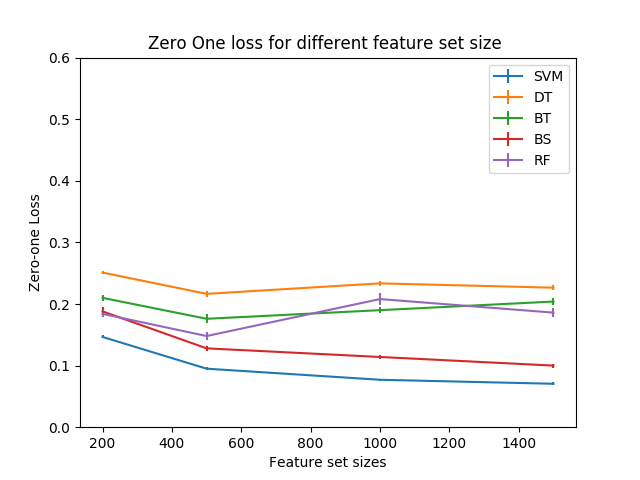
\includegraphics{Analysis2.png}
\end{figure}

\subsection{Hypothesis}

Let's compare SVM with RF. 

Null hypothesis is that both are equivalent in terms of performance. This means that the 
mean of the SVM 0/1 losses is equivalent to the mean of the RF 0/1 losses. It is assumed
to be true. 

While the alternative hypothesis is that SVM and RF zero one losses are significantly different.
Or, that the mean of the SVM zero one losses is lesser than the mean of the RF 0/1 losses.

\subsection{Discussion to test the hypothesis}

It can be seen from the average zero one loss and standard error values for the two algorithms
that the differences are significant. The plots do not overlap each other.

We perform t-test to compare the performance. The results for different feature set sizes are given below:

For 200 feature set size:
  The two-tailed P value equals 0.0010   \\

For 500 feature set size:
  The two-tailed P value equals 0.0035   \\

For 1000 feature set size:
  The two-tailed P value equals 0.0019    \\

For 1500 feature set size:
  The two-tailed P value equals 0.0012   \\

Since p values are always lesser than 0.05 / 4 = 0.0125 therefore null is rejected and we
conclude SVM mean losses are lesser than RF.

\section{Analysis 3}

\subsection{Learning Curves}

In this analysis we vary the depth limit of the trees in DT, and its ensembles. 
The comparative result while varying number of features is shown in Figure 3.

On x-axis we vary the depth of the tree. On y-axis is the zero one loss. 
We have five plots --- one for each model with different color. The vertical 
bars show the standard error calculated as described in the homework handout. The 
values of zero one loss for each of the four depth limits averaged accross 10 fold for 
each of the five models along with the corresponding standard errors are given below. The
first array shows the average 0/1 losses while the second array shows the corresponding 
standard errors.
\\
=======SVM======\\

[0.07150000000000001, 0.078, 0.07100000000000001, 0.07500000000000002]

[0.0015337861650177966, 0.001345362404707371, 0.0011789826122551598, 0.0014317821063276352]

=======DT======\\

[0.28450000000000003, 0.23500000000000001, 0.192, 0.22950000000000004]

[0.0047457876058669126, 0.0048114446894877635, 0.0044000000000000003, 0.0026781523481684165]

=======BT======\\

[0.238, 0.16, 0.16599999999999998, 0.158]

[0.0070682388188289171, 0.0080000000000000002, 0.008002499609497022, 0.0060959002616512688]

=======RF======\\

[0.314, 0.18200000000000005, 0.15400000000000003, 0.12200000000000003]

[0.0071582120672693123, 0.0089643739324059887, 0.0072691127381544996, 0.0047707441767506258]

=======BS======\\

[0.094, 0.08199999999999999, 0.098, 0.10199999999999998]

[0.0044766058571198784, 0.0036276714294434112, 0.0045122056690713921, 0.0070682388188289163]


The above values are calculated from the following zero one loss values for varying training
set size each having10 folds:
\\
=======================================
ZERO-ONE-LOSS-DT 0.33
ZERO-ONE-LOSS-BT 0.26
ZERO-ONE-LOSS-RF 0.32
ZERO-ONE-LOSS-BS 0.08
ZERO-ONE-LOSS-SVM 0.075
ZERO-ONE-LOSS-DT 0.25
ZERO-ONE-LOSS-BT 0.22
ZERO-ONE-LOSS-RF 0.34
ZERO-ONE-LOSS-BS 0.12
ZERO-ONE-LOSS-SVM 0.07
ZERO-ONE-LOSS-DT 0.38
ZERO-ONE-LOSS-BT 0.26
ZERO-ONE-LOSS-RF 0.26
ZERO-ONE-LOSS-BS 0.14
ZERO-ONE-LOSS-SVM 0.085
ZERO-ONE-LOSS-DT 0.335
ZERO-ONE-LOSS-BT 0.34
ZERO-ONE-LOSS-RF 0.38
ZERO-ONE-LOSS-BS 0.1
ZERO-ONE-LOSS-SVM 0.08
ZERO-ONE-LOSS-DT 0.245
ZERO-ONE-LOSS-BT 0.18
ZERO-ONE-LOSS-RF 0.34
ZERO-ONE-LOSS-BS 0.08
ZERO-ONE-LOSS-SVM 0.065
ZERO-ONE-LOSS-DT 0.24
ZERO-ONE-LOSS-BT 0.14
ZERO-ONE-LOSS-RF 0.36
ZERO-ONE-LOSS-BS 0.04
ZERO-ONE-LOSS-SVM 0.035
ZERO-ONE-LOSS-DT 0.275
ZERO-ONE-LOSS-BT 0.3
ZERO-ONE-LOSS-RF 0.42
ZERO-ONE-LOSS-BS 0.16
ZERO-ONE-LOSS-SVM 0.075
ZERO-ONE-LOSS-DT 0.24
ZERO-ONE-LOSS-BT 0.2
ZERO-ONE-LOSS-RF 0.24
ZERO-ONE-LOSS-BS 0.1
ZERO-ONE-LOSS-SVM 0.095
ZERO-ONE-LOSS-DT 0.305
ZERO-ONE-LOSS-BT 0.34
ZERO-ONE-LOSS-RF 0.32
ZERO-ONE-LOSS-BS 0.12
ZERO-ONE-LOSS-SVM 0.075
ZERO-ONE-LOSS-DT 0.245
ZERO-ONE-LOSS-BT 0.14
ZERO-ONE-LOSS-RF 0.16
ZERO-ONE-LOSS-BS 0.0
ZERO-ONE-LOSS-SVM 0.06
=======================================
ZERO-ONE-LOSS-DT 0.26
ZERO-ONE-LOSS-BT 0.2
ZERO-ONE-LOSS-RF 0.12
ZERO-ONE-LOSS-BS 0.12
ZERO-ONE-LOSS-SVM 0.085
ZERO-ONE-LOSS-DT 0.195
ZERO-ONE-LOSS-BT 0.2
ZERO-ONE-LOSS-RF 0.14
ZERO-ONE-LOSS-BS 0.04
ZERO-ONE-LOSS-SVM 0.09
ZERO-ONE-LOSS-DT 0.295
ZERO-ONE-LOSS-BT 0.22
ZERO-ONE-LOSS-RF 0.32
ZERO-ONE-LOSS-BS 0.1
ZERO-ONE-LOSS-SVM 0.105
ZERO-ONE-LOSS-DT 0.31
ZERO-ONE-LOSS-BT 0.28
ZERO-ONE-LOSS-RF 0.14
ZERO-ONE-LOSS-BS 0.14
ZERO-ONE-LOSS-SVM 0.085
ZERO-ONE-LOSS-DT 0.225
ZERO-ONE-LOSS-BT 0.06
ZERO-ONE-LOSS-RF 0.2
ZERO-ONE-LOSS-BS 0.1
ZERO-ONE-LOSS-SVM 0.06
ZERO-ONE-LOSS-DT 0.24
ZERO-ONE-LOSS-BT 0.12
ZERO-ONE-LOSS-RF 0.26
ZERO-ONE-LOSS-BS 0.08
ZERO-ONE-LOSS-SVM 0.08
ZERO-ONE-LOSS-DT 0.15
ZERO-ONE-LOSS-BT 0.06
ZERO-ONE-LOSS-RF 0.08
ZERO-ONE-LOSS-BS 0.1
ZERO-ONE-LOSS-SVM 0.075
ZERO-ONE-LOSS-DT 0.18
ZERO-ONE-LOSS-BT 0.04
ZERO-ONE-LOSS-RF 0.08
ZERO-ONE-LOSS-BS 0.02
ZERO-ONE-LOSS-SVM 0.065
ZERO-ONE-LOSS-DT 0.225
ZERO-ONE-LOSS-BT 0.18
ZERO-ONE-LOSS-RF 0.14
ZERO-ONE-LOSS-BS 0.04
ZERO-ONE-LOSS-SVM 0.06
ZERO-ONE-LOSS-DT 0.27
ZERO-ONE-LOSS-BT 0.24
ZERO-ONE-LOSS-RF 0.34
ZERO-ONE-LOSS-BS 0.08
ZERO-ONE-LOSS-SVM 0.075
=======================================
ZERO-ONE-LOSS-DT 0.18
ZERO-ONE-LOSS-BT 0.22
ZERO-ONE-LOSS-RF 0.28
ZERO-ONE-LOSS-BS 0.06
ZERO-ONE-LOSS-SVM 0.075
ZERO-ONE-LOSS-DT 0.22
ZERO-ONE-LOSS-BT 0.24
ZERO-ONE-LOSS-RF 0.1
ZERO-ONE-LOSS-BS 0.1
ZERO-ONE-LOSS-SVM 0.085
ZERO-ONE-LOSS-DT 0.26
ZERO-ONE-LOSS-BT 0.26
ZERO-ONE-LOSS-RF 0.2
ZERO-ONE-LOSS-BS 0.16
ZERO-ONE-LOSS-SVM 0.065
ZERO-ONE-LOSS-DT 0.195
ZERO-ONE-LOSS-BT 0.22
ZERO-ONE-LOSS-RF 0.14
ZERO-ONE-LOSS-BS 0.14
ZERO-ONE-LOSS-SVM 0.085
ZERO-ONE-LOSS-DT 0.155
ZERO-ONE-LOSS-BT 0.02
ZERO-ONE-LOSS-RF 0.02
ZERO-ONE-LOSS-BS 0.08
ZERO-ONE-LOSS-SVM 0.065
ZERO-ONE-LOSS-DT 0.22
ZERO-ONE-LOSS-BT 0.16
ZERO-ONE-LOSS-RF 0.2
ZERO-ONE-LOSS-BS 0.14
ZERO-ONE-LOSS-SVM 0.08
ZERO-ONE-LOSS-DT 0.23
ZERO-ONE-LOSS-BT 0.2
ZERO-ONE-LOSS-RF 0.22
ZERO-ONE-LOSS-BS 0.04
ZERO-ONE-LOSS-SVM 0.08
ZERO-ONE-LOSS-DT 0.125
ZERO-ONE-LOSS-BT 0.02
ZERO-ONE-LOSS-RF 0.12
ZERO-ONE-LOSS-BS 0.02
ZERO-ONE-LOSS-SVM 0.065
ZERO-ONE-LOSS-DT 0.215
ZERO-ONE-LOSS-BT 0.16
ZERO-ONE-LOSS-RF 0.18
ZERO-ONE-LOSS-BS 0.14
ZERO-ONE-LOSS-SVM 0.065
ZERO-ONE-LOSS-DT 0.12
ZERO-ONE-LOSS-BT 0.16
ZERO-ONE-LOSS-RF 0.08
ZERO-ONE-LOSS-BS 0.1
ZERO-ONE-LOSS-SVM 0.045
=======================================
ZERO-ONE-LOSS-DT 0.25
ZERO-ONE-LOSS-BT 0.16
ZERO-ONE-LOSS-RF 0.14
ZERO-ONE-LOSS-BS 0.04
ZERO-ONE-LOSS-SVM 0.075
ZERO-ONE-LOSS-DT 0.21
ZERO-ONE-LOSS-BT 0.12
ZERO-ONE-LOSS-RF 0.04
ZERO-ONE-LOSS-BS 0.12
ZERO-ONE-LOSS-SVM 0.095
ZERO-ONE-LOSS-DT 0.265
ZERO-ONE-LOSS-BT 0.26
ZERO-ONE-LOSS-RF 0.16
ZERO-ONE-LOSS-BS 0.3
ZERO-ONE-LOSS-SVM 0.095
ZERO-ONE-LOSS-DT 0.19
ZERO-ONE-LOSS-BT 0.28
ZERO-ONE-LOSS-RF 0.18
ZERO-ONE-LOSS-BS 0.1
ZERO-ONE-LOSS-SVM 0.07
ZERO-ONE-LOSS-DT 0.26
ZERO-ONE-LOSS-BT 0.14
ZERO-ONE-LOSS-RF 0.12
ZERO-ONE-LOSS-BS 0.1
ZERO-ONE-LOSS-SVM 0.09
ZERO-ONE-LOSS-DT 0.225
ZERO-ONE-LOSS-BT 0.14
ZERO-ONE-LOSS-RF 0.12
ZERO-ONE-LOSS-BS 0.08
ZERO-ONE-LOSS-SVM 0.07
ZERO-ONE-LOSS-DT 0.265
ZERO-ONE-LOSS-BT 0.16
ZERO-ONE-LOSS-RF 0.2
ZERO-ONE-LOSS-BS 0.1
ZERO-ONE-LOSS-SVM 0.08
ZERO-ONE-LOSS-DT 0.21
ZERO-ONE-LOSS-BT 0.08
ZERO-ONE-LOSS-RF 0.1
ZERO-ONE-LOSS-BS 0.04
ZERO-ONE-LOSS-SVM 0.065
ZERO-ONE-LOSS-DT 0.2
ZERO-ONE-LOSS-BT 0.14
ZERO-ONE-LOSS-RF 0.1
ZERO-ONE-LOSS-BS 0.08
ZERO-ONE-LOSS-SVM 0.06
ZERO-ONE-LOSS-DT 0.22
ZERO-ONE-LOSS-BT 0.1
ZERO-ONE-LOSS-RF 0.06
ZERO-ONE-LOSS-BS 0.06
ZERO-ONE-LOSS-SVM 0.05

\begin{figure}
	\centering
	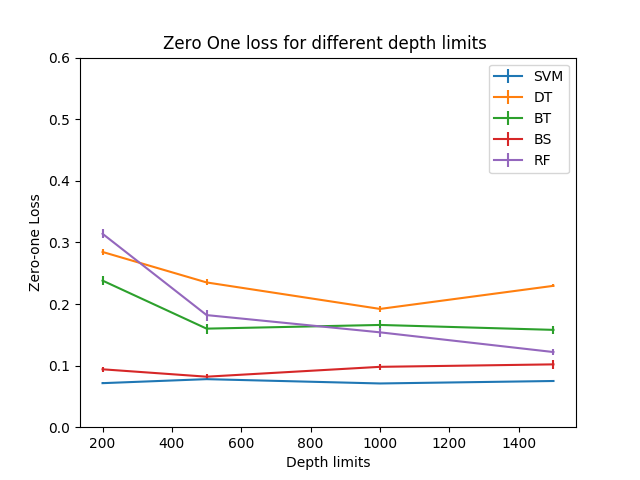
\includegraphics{Analysis3.png}
\end{figure}

\subsection{Hypothesis}

Let's compare BT with DT. 

Null hypothesis is that both are equivalent in terms of performance. That is the mean of the
zero one losses of BT is equivalent to the mean of the zero one losses of the DT. It is assumed
to be true. 

While the alternative hypothesis is that BT and DT zero one losses are significantly different.
Or, that the mean of the BT zero one losses is lesser than the mean of the DT 0/1 losses.
This is because the ensemble BT reduces error due to variance.

\subsection{Discussion to test the hypothesis}

We perform t-test to compare the performance. The results for different depths are given below:

For 5 depth:
  The two-tailed P value equals 0.0256   \\

For 10 depth:
  The two-tailed P value equals 0.0017   \\

For 15 depth:
  The two-tailed P value equals 0.0325    \\

For 20 depth:
  The two-tailed P value equals 0.0019   \\

From the above testing it can be seen that null is rejected only in two cases (10 and 20).
While it is accepted for 5 and 15 depths.  Null is only rejected when p values is less than 0.0125.

\section{Analysis 4}

\subsection{Learning Curves}

In this analysis we vary the number of trees in ensembles of DT.
The comparative result while varying number of features is shown in Figure 4.

On x-axis we vary the number of trees considered. On y-axis is the zero one loss. 
We have five plots --- one for each model with different color. The vertical 
bars show the standard error calculated as described in the homework handout. The 
values of zero one loss for each of the four different numbers of trees averaged accross 10 fold for 
each of the five models along with the corresponding standard errors are given below. The
first array shows the average 0/1 losses while the second array shows the corresponding 
standard errors.
\\
=======SVM======

[0.0705, 0.076, 0.0685, 0.08049999999999999]

[0.0017811513130556876, 0.0023537204591879642, 0.0011412712210513327, 0.0015402921800749363]

=======DT======

[0.23149999999999996, 0.205, 0.202, 0.2125]

[0.0041173413752080366, 0.0031064449134018133, 0.0015198684153570658, 0.0033335416601566565]

=======BT======

[0.25, 0.172, 0.178, 0.187]

[0.017464249196572978, 0.0047497368348151676, 0.0067793805026713184, 0.0044732538492690075]

=======RF======

[0.28, 0.184, 0.14600000000000005, 0.14800000000000002]

[0.015362291495737219, 0.0086162636914152053, 0.0042000000000000006, 0.0059126981996377934]

=======BS======

[0.14, 0.11200000000000002, 0.09600000000000002, 0.08800000000000001]

[0.010198039027185571, 0.0064000000000000003, 0.0041761226035642203, 0.0026758176320519299]


The above values are calculated from the following zero one loss values for varying training
set size each having10 folds:
\\

=======================================
ZERO-ONE-LOSS-DT 0.315
ZERO-ONE-LOSS-BT 0.5
ZERO-ONE-LOSS-RF 0.5
ZERO-ONE-LOSS-BS 0.3
ZERO-ONE-LOSS-SVM 0.065
ZERO-ONE-LOSS-DT 0.235
ZERO-ONE-LOSS-BT 0.2
ZERO-ONE-LOSS-RF 0.4
ZERO-ONE-LOSS-BS 0.3
ZERO-ONE-LOSS-SVM 0.09
ZERO-ONE-LOSS-DT 0.18
ZERO-ONE-LOSS-BT 0.1
ZERO-ONE-LOSS-RF 0.1
ZERO-ONE-LOSS-BS 0.1
ZERO-ONE-LOSS-SVM 0.07
ZERO-ONE-LOSS-DT 0.205
ZERO-ONE-LOSS-BT 0.3
ZERO-ONE-LOSS-RF 0.3
ZERO-ONE-LOSS-BS 0.1
ZERO-ONE-LOSS-SVM 0.09
ZERO-ONE-LOSS-DT 0.245
ZERO-ONE-LOSS-BT 0.6
ZERO-ONE-LOSS-RF 0.1
ZERO-ONE-LOSS-BS 0.2
ZERO-ONE-LOSS-SVM 0.07
ZERO-ONE-LOSS-DT 0.23
ZERO-ONE-LOSS-BT 0.3
ZERO-ONE-LOSS-RF 0.1
ZERO-ONE-LOSS-BS 0.0
ZERO-ONE-LOSS-SVM 0.05
ZERO-ONE-LOSS-DT 0.18
ZERO-ONE-LOSS-BT 0.1
ZERO-ONE-LOSS-RF 0.1
ZERO-ONE-LOSS-BS 0.1
ZERO-ONE-LOSS-SVM 0.085
ZERO-ONE-LOSS-DT 0.275
ZERO-ONE-LOSS-BT 0.0
ZERO-ONE-LOSS-RF 0.4
ZERO-ONE-LOSS-BS 0.0
ZERO-ONE-LOSS-SVM 0.08
ZERO-ONE-LOSS-DT 0.195
ZERO-ONE-LOSS-BT 0.2
ZERO-ONE-LOSS-RF 0.4
ZERO-ONE-LOSS-BS 0.1
ZERO-ONE-LOSS-SVM 0.03
ZERO-ONE-LOSS-DT 0.255
ZERO-ONE-LOSS-BT 0.2
ZERO-ONE-LOSS-RF 0.4
ZERO-ONE-LOSS-BS 0.2
ZERO-ONE-LOSS-SVM 0.075
=======================================
ZERO-ONE-LOSS-DT 0.185
ZERO-ONE-LOSS-BT 0.16
ZERO-ONE-LOSS-RF 0.04
ZERO-ONE-LOSS-BS 0.16
ZERO-ONE-LOSS-SVM 0.075
ZERO-ONE-LOSS-DT 0.225
ZERO-ONE-LOSS-BT 0.24
ZERO-ONE-LOSS-RF 0.28
ZERO-ONE-LOSS-BS 0.08
ZERO-ONE-LOSS-SVM 0.135
ZERO-ONE-LOSS-DT 0.155
ZERO-ONE-LOSS-BT 0.2
ZERO-ONE-LOSS-RF 0.12
ZERO-ONE-LOSS-BS 0.12
ZERO-ONE-LOSS-SVM 0.07
ZERO-ONE-LOSS-DT 0.21
ZERO-ONE-LOSS-BT 0.2
ZERO-ONE-LOSS-RF 0.36
ZERO-ONE-LOSS-BS 0.24
ZERO-ONE-LOSS-SVM 0.095
ZERO-ONE-LOSS-DT 0.25
ZERO-ONE-LOSS-BT 0.08
ZERO-ONE-LOSS-RF 0.16
ZERO-ONE-LOSS-BS 0.0
ZERO-ONE-LOSS-SVM 0.05
ZERO-ONE-LOSS-DT 0.225
ZERO-ONE-LOSS-BT 0.12
ZERO-ONE-LOSS-RF 0.24
ZERO-ONE-LOSS-BS 0.12
ZERO-ONE-LOSS-SVM 0.08
ZERO-ONE-LOSS-DT 0.18
ZERO-ONE-LOSS-BT 0.2
ZERO-ONE-LOSS-RF 0.2
ZERO-ONE-LOSS-BS 0.08
ZERO-ONE-LOSS-SVM 0.075
ZERO-ONE-LOSS-DT 0.25
ZERO-ONE-LOSS-BT 0.2
ZERO-ONE-LOSS-RF 0.12
ZERO-ONE-LOSS-BS 0.16
ZERO-ONE-LOSS-SVM 0.07
ZERO-ONE-LOSS-DT 0.17
ZERO-ONE-LOSS-BT 0.2
ZERO-ONE-LOSS-RF 0.16
ZERO-ONE-LOSS-BS 0.12
ZERO-ONE-LOSS-SVM 0.05
ZERO-ONE-LOSS-DT 0.2
ZERO-ONE-LOSS-BT 0.12
ZERO-ONE-LOSS-RF 0.16
ZERO-ONE-LOSS-BS 0.04
ZERO-ONE-LOSS-SVM 0.06
=======================================
ZERO-ONE-LOSS-DT 0.17
ZERO-ONE-LOSS-BT 0.14
ZERO-ONE-LOSS-RF 0.12
ZERO-ONE-LOSS-BS 0.14
ZERO-ONE-LOSS-SVM 0.065
ZERO-ONE-LOSS-DT 0.205
ZERO-ONE-LOSS-BT 0.2
ZERO-ONE-LOSS-RF 0.22
ZERO-ONE-LOSS-BS 0.08
ZERO-ONE-LOSS-SVM 0.09
ZERO-ONE-LOSS-DT 0.19
ZERO-ONE-LOSS-BT 0.1
ZERO-ONE-LOSS-RF 0.14
ZERO-ONE-LOSS-BS 0.08
ZERO-ONE-LOSS-SVM 0.055
ZERO-ONE-LOSS-DT 0.235
ZERO-ONE-LOSS-BT 0.22
ZERO-ONE-LOSS-RF 0.12
ZERO-ONE-LOSS-BS 0.08
ZERO-ONE-LOSS-SVM 0.07
ZERO-ONE-LOSS-DT 0.205
ZERO-ONE-LOSS-BT 0.14
ZERO-ONE-LOSS-RF 0.22
ZERO-ONE-LOSS-BS 0.08
ZERO-ONE-LOSS-SVM 0.085
ZERO-ONE-LOSS-DT 0.205
ZERO-ONE-LOSS-BT 0.28
ZERO-ONE-LOSS-RF 0.16
ZERO-ONE-LOSS-BS 0.16
ZERO-ONE-LOSS-SVM 0.07
ZERO-ONE-LOSS-DT 0.205
ZERO-ONE-LOSS-BT 0.18
ZERO-ONE-LOSS-RF 0.14
ZERO-ONE-LOSS-BS 0.1
ZERO-ONE-LOSS-SVM 0.06
ZERO-ONE-LOSS-DT 0.205
ZERO-ONE-LOSS-BT 0.18
ZERO-ONE-LOSS-RF 0.12
ZERO-ONE-LOSS-BS 0.04
ZERO-ONE-LOSS-SVM 0.075
ZERO-ONE-LOSS-DT 0.2
ZERO-ONE-LOSS-BT 0.28
ZERO-ONE-LOSS-RF 0.14
ZERO-ONE-LOSS-BS 0.16
ZERO-ONE-LOSS-SVM 0.055
ZERO-ONE-LOSS-DT 0.2
ZERO-ONE-LOSS-BT 0.06
ZERO-ONE-LOSS-RF 0.08
ZERO-ONE-LOSS-BS 0.04
ZERO-ONE-LOSS-SVM 0.06
=======================================
ZERO-ONE-LOSS-DT 0.23
ZERO-ONE-LOSS-BT 0.18
ZERO-ONE-LOSS-RF 0.11
ZERO-ONE-LOSS-BS 0.12
ZERO-ONE-LOSS-SVM 0.075
ZERO-ONE-LOSS-DT 0.16
ZERO-ONE-LOSS-BT 0.24
ZERO-ONE-LOSS-RF 0.18
ZERO-ONE-LOSS-BS 0.11
ZERO-ONE-LOSS-SVM 0.1
ZERO-ONE-LOSS-DT 0.225
ZERO-ONE-LOSS-BT 0.12
ZERO-ONE-LOSS-RF 0.07
ZERO-ONE-LOSS-BS 0.06
ZERO-ONE-LOSS-SVM 0.06
ZERO-ONE-LOSS-DT 0.205
ZERO-ONE-LOSS-BT 0.15
ZERO-ONE-LOSS-RF 0.28
ZERO-ONE-LOSS-BS 0.12
ZERO-ONE-LOSS-SVM 0.09
ZERO-ONE-LOSS-DT 0.255
ZERO-ONE-LOSS-BT 0.24
ZERO-ONE-LOSS-RF 0.16
ZERO-ONE-LOSS-BS 0.07
ZERO-ONE-LOSS-SVM 0.1
ZERO-ONE-LOSS-DT 0.185
ZERO-ONE-LOSS-BT 0.16
ZERO-ONE-LOSS-RF 0.19
ZERO-ONE-LOSS-BS 0.05
ZERO-ONE-LOSS-SVM 0.05
ZERO-ONE-LOSS-DT 0.165
ZERO-ONE-LOSS-BT 0.19
ZERO-ONE-LOSS-RF 0.16
ZERO-ONE-LOSS-BS 0.11
ZERO-ONE-LOSS-SVM 0.075
ZERO-ONE-LOSS-DT 0.245
ZERO-ONE-LOSS-BT 0.21
ZERO-ONE-LOSS-RF 0.14
ZERO-ONE-LOSS-BS 0.11
ZERO-ONE-LOSS-SVM 0.085
ZERO-ONE-LOSS-DT 0.255
ZERO-ONE-LOSS-BT 0.25
ZERO-ONE-LOSS-RF 0.12
ZERO-ONE-LOSS-BS 0.07
ZERO-ONE-LOSS-SVM 0.08
ZERO-ONE-LOSS-DT 0.2
ZERO-ONE-LOSS-BT 0.13
ZERO-ONE-LOSS-RF 0.07
ZERO-ONE-LOSS-BS 0.06
ZERO-ONE-LOSS-SVM 0.09

\begin{figure}
	\centering
	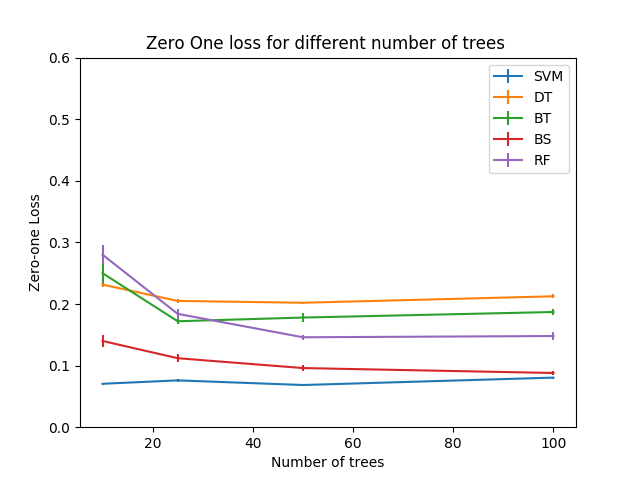
\includegraphics{Analysis4.png}
\end{figure}

\subsection{Hypothesis}

Let's compare RF with DT. 

Null hypothesis is that both are equivalent in terms of performance. That is the mean of the
zero one losses of RF is equivalent to the mean of the zero one losses of the DT. It is assumed
to be true. 

While the alternative hypothesis is that RF and DT zero one losses are significantly different.
Or, that the mean of the RF zero one losses is lesser than the mean of the DT 0/1 losses.
This is because the ensemble RF reduces error due to variance.

\subsection{Discussion to test the hypothesis}

We perform t-test to compare the performance. The results for different number of trees are given below:

For 10:
  The two-tailed P value equals 0.3017   \\

For 25:
  The two-tailed P value equals 0.4728   \\

For 50:
  The two-tailed P value equals 0.3599    \\

For 100:
  The two-tailed P value equals 0.0343   \\

Since the p values are always greater than 0.0125 we conclude that null is accepted.

\newpage 

\section{Bonus part}

Boosted decision trees (BS) are also implemented using the tutorial mentioned at:

https://engineering.purdue.edu/kak/Tutorials/AdaBoost.pdf

The results are included in the figures mentioned above.

\subsection{Hypothesis 1}

Let's compare SVM with BS using cross validation on training set sizes.

Null hypothesis is that both are equivalent in terms of performance. That is the mean of the
zero one losses of SVM is equivalent to the mean of the zero one losses of the BS. It is assumed
to be true. 

While the alternative hypothesis is that SVM and BS zero one losses are significantly different.
Or, that the mean of the SVM zero one losses is lesser than the mean of the BS 0/1 losses.

\subsection{Discussion to test the hypothesis 1}

We perform t-test to compare the performance. The results for different training set sizes are given below:
For training percents of [2.5, 5, 12.5, 25] p values are 0.0182, 0.8287, 0.0107, 0.435   \\

Sometimes null is accepted and sometimes it is rejected. It depends on whether the p values is 
less than 0.0125 or greater than 0.0125. If p is less than 0.0125 null is rejected.

\subsection{Hypothesis 1}

Let's compare BS with RF while doing cross validation on traininig set size.

Null hypothesis is that both are equivalent in terms of performance. That is the mean of the
zero one losses of RF is equivalent to the mean of the zero one losses of the BS. It is assumed
to be true. 

While the alternative hypothesis is that RF and BS zero one losses are significantly different.
Or, that the mean of the BS zero one losses is lesser than the mean of the RF 0/1 losses.

\subsection{Discussion to test the hypothesis 1}

We perform t-test to compare the performance. The results for different training set sizes are given below:

For 2.5:
  The two-tailed P value equals 0.0292  \\

For 5:
  The two-tailed P value equals 0.0002   \\

For 12.5:
  The two-tailed P value equals 0.6899    \\

For 25:
  The two-tailed P value equals 0.0343   \\


Sometimes null is accepted and sometimes it is rejected. It depends on whether the p values is 
less than 0.0125 or greater than 0.0125. If p is less than 0.0125 null is rejected.

\section{Decomposition}

If h(x) is the prediction label of an example x and y is true label.
Then expected mean squared error is:

\begin{equation}
E[MSE] = E[y-h(x)]^2
\end{equation}

We need to decompose this into noise, bias, and variance.

\begin{equation}
 E[(h(x) -y)^2] = E[h(x)^2 -2h(x)y + y^2] = E[h(x)^2] -2 E[h(x)] E[y] +E[y]
\end{equation}

We know that:

\begin{equation}
E[Z^2] = E[(Z-Z^*)^2] + Z^{*2}
\end{equation}

where Z is a random variable and $Z^*$ is the mean of Z. 

Therefore,

\begin{equation}
 E[(h(x) -y)^2]  = E[h(x) - h(x)^*] + h(x)^{*2} - 2 h(x)^* f(x) + E[(f(x) -y)^2] + f(x)^2
\end{equation}

\begin{equation}
= E[(h(x) - h(x)^*)^2] + (h(x) - f(x))^2 + E[(f(x) - y)^2]
\end{equation}

\begin{equation}
= Variance + bias^2 + noise
\end{equation}

\end{document}